\documentclass[11pt]{article} % or another document class of your choice

% Packages

% \usepackage[backend=biber, style=authoryear]{biblatex}  
% \addbibresource{references.bib}
\usepackage{authblk}  % For author affiliations
\usepackage[utf8]{inputenc}      % Encoding of the document
\usepackage[T1]{fontenc}         % Font encoding
\usepackage{xcolor}
\usepackage{amsmath, amssymb, amsthm} % Math packages
\usepackage{graphicx}            % For including graphics
\usepackage{hyperref}            % For hyperlinks
\usepackage{pgfplots}
\pgfplotsset{compat=1.18}
\usepackage{siunitx} % For aligning numbers in tables
\usepackage{float}
\usepackage{geometry}            % To adjust page dimensions
\usepackage{booktabs}
\geometry{margin=1in}            % Set margins


\title{\textbf{Towards Enterprise-Ready Computer Using Generalist Agent}}

\author{\textbf{Sami Marreed}$^{*}$, \textbf{Alon Oved}$^{*}$, \textbf{Avi Yaeli}$^{*}$, \textbf{Segev Shlomov}$^{*}$, \textbf{Ido Levy}, \textbf{Aviad Sela}, \textbf{Asaf Adi}, \textbf{Nir Mashkif}}

\affil{\small IBM Research}

\affil{\small \texttt{\{sami.marreed, alon.oved, segev.shlomov1, ido.levy1\}@ibm.com}}

\affil{\small \texttt{\{aviy, sela, adi, nirm\}@il.ibm.com}} 

% \author{
%     Sami Marreed\textsuperscript{\rm *}, Alon Oved\textsuperscript{\rm *}, Avi Yaeli\textsuperscript{\rm *}, Segev Shlomov, Ido Levy, \\Aviad Sela, Asaf Adi, Nir Mashkif\\
%     \\
%     IBM Research\\
%     \textsuperscript{*}Lead contributors.\\
%     \{sami.marreed, alon.oved, segev.shlomov1, ido.levy1\}@ibm.com\\
%     \{aviy, sela, adi, nirm\}@il.ibm.com
% } 

 
\date{}


\begin{document}


\maketitle

\begingroup
\renewcommand\thefootnote{}\footnotetext{*These lead authors  contributed equally to this work}
\endgroup

\begin{abstract}
This paper presents our ongoing work toward developing an enterprise-ready Computer Using Generalist Agent (CUGA) system.  Our research highlights the evolutionary nature of building agentic systems suitable for enterprise environments. By integrating state-of-the-art agentic AI techniques with a systematic approach to iterative evaluation, analysis, and refinement, we have achieved rapid and cost-effective performance gains, notably reaching a new state-of-the-art performance on the WebArena benchmark. We detail our development roadmap, the methodology and tools that facilitated rapid learning from failures and continuous system refinement, and discuss key lessons learned and future challenges for enterprise adoption.
% \textcolor{blue}{
% architecture updates, arxiv, , author workbench, , 
% }
% TBD - add footnote(DONE), emails(DONE), Aviad(DONE), errors(DONE), lifecycle arrow (Done), Iteration --> Runs (DONE), web browser--> web application(DONE), consider to remove w/o requiring technical support (DONE, search manner), At IBM --> At IBM Research (DONE); business user --> knoweldge worker, . add IBM's plan for safety and human-in-the-loop, 

\end{abstract}

\section{Introduction}

The development of enterprise-ready, computer-using generalist agents represents a significant frontier in artificial intelligence, poised to revolutionize productivity, workflows, automation, and decision-making across diverse industries.  Recent advances in large language, vision, and action models, coupled with progress in agentic AI frameworks and implementations, are continuously raising the bar on existing computer-using benchmarks.  While recent announcements, such as Anthropic's Computer Use \cite{anthropicComputerUse2024} and OpenAI's Operator \cite{openaiOperator2025}, suggest a growing commercial opportunity, realizing this vision requires more than just cutting-edge models, algorithms, or product prototypes, and significant challenges still remain.

At IBM Research, our ambition is to pioneer the development of agent systems that transcend mere task completion, and encompass the full spectrum of dimensions required for enterprise adoption, such as privacy, safety, trustworthiness, and cost-effectiveness of AI agentic solutions.  As part of this mission, we have begun to develop a Computer Using Generalist Agent (CUGA).  Our vision for IBM CUGA is to develop a generalist agent that can be adapted and configured by knowledge workers to perform routine or complex aspects of their work in a safe and trustworthy manner. Our first version focuses on knowledge worker tasks within web applications, and we tested it on the WebArena benchmark \cite{zhou2023webarena}. On WebArena, our agent achieves a new state of the art result of 61.7\% on task completion \cite{wearena_leaderboard}.
% powered by our multi-agent architecture and using GPT-4o as the backend model.  

This paper details the current state of our work, outlining the evolution of our agentic architecture to address the challenges posed by the WebArena benchmark. We describe our iterative development methodology and the tools that facilitated rapid learning from failures and cost-effective architectural improvements.  Furthermore, we share lessons learned and highlight key challenges in realizing the full potential of such systems. Our primary contribution lies in disseminating the methodology, architecture, and practical experience that enabled us to achieve top performance on the WebArena leaderboard.  Additionally, we have created a fully interactive dashboard \footnote{IBM CUGA dashboard - https://cuga.dev/} showcasing our performance results and agent trajectories, enhancing transparency.  

\section{Methodology and Tools}

Our approach to developing an enterprise-ready computer using generalist agent (CUGA) is grounded in a philosophy of iterative evolution and rapid learning. We began with a simple agent architecture, intentionally designed to be a starting point, and committed to refining it based on empirical results and failure analysis. This evolutionary strategy allows us to adapt quickly to the complexities of real-world scenarios and continuously improve performance.

A cornerstone of our development methodology is the implementation of a smart sampling strategy. Recognizing the time-intensive nature of evaluating agent systems on comprehensive benchmarks, we adopted a technique of selecting an initially small, representative subset of the benchmark, enlarging the subsets as the system evolved to be better and more stable. This allowed us to rapidly test hypotheses, identify failure areas and side effects, and iterate on improvements before scaling up to larger portions of the benchmark. This approach significantly accelerates our learning cycle, enabling us to achieve rapid performance gains.  Figure \ref{fig:cuga_lifecycle} depicts the main phases in our iterative evaluate-analyze-enhance process.  In each iteration we evaluate on a larger sample, validate that expected performance gains are achieved, we analyze failures and prioritize areas of improvements that would maximize the performance gain in the following cycle.
 

\begin{figure}[htbp]
    \centering
    \includegraphics[width=1.0\textwidth]{images/Lifecycle.png}
    \caption{The evaluate-analyze-enhance iterative development process.}  
    \label{fig:cuga_lifecycle}
\end{figure}

To facilitate this iterative process, we developed a suite of evaluation and analysis tools designed to provide comprehensive insights and accelerate development:



% \begin{figure}[htbp]  
\begin{figure}[H]
    \centering
    \includegraphics[width=\textwidth]{images/CUGA-Dashboard.png}
    \caption{CUGA performance dashboard providing an overview and details performance results per task, with drill down links into trajectories}
    \label{fig:cuga_dashboard} 
\end{figure}

\begin{enumerate}
    \item \textbf{Performance Dashboard:} This dashboard, as depicted by Figure \ref{fig:cuga_dashboard} provides a real-time overview of the agent's performance across various metrics. It allows us to quickly assess the impact of new versions and identify areas for improvement.
    \item \textbf{Comparative Analysis:} Building upon the performance dashboard, this view enables direct comparison of results between different agent versions. It highlights previously resolved failures that are now successful, new failures on new data points, as well as failures on previously successful runs.  This feature allows for rapid assessment of the impact of changes, validation of hypotheses, detection of side effects, and for regression purposes.  
    \item \textbf{Trajectory Visualization and error classification:} This tool, depicted in Figure \ref{fig:cuga_trajectory} allows us to delve into individual failure cases, visualizing the agent's interaction with the environment, its perception, reasoning process, and actions taken by different components. This detailed view enables us to quickly pinpoint and classify the root cause of failures and generate targeted hypotheses for improvement.
    \item \textbf{Parallel Execution Framework:} To significantly reduce evaluation time, we implemented a parallel execution framework. This framework allows us to run multiple evaluations concurrently, reducing evaluation times from days to hours, and from hours to minutes. This speedup is crucial for rapid iteration and experimentation.
\end{enumerate}


% \begin{figure}[htbp]  
\begin{figure}[H]
    \centering
    \includegraphics[width=0.6\textwidth]{images/Trajectory-Visualization.png}
    \caption{The CUGA trajectory visualization, provides an easy access to the environment observation as screenshot, perception as accessibility tree, the action instruction, and its element grounding in the accessibility tree}
    \label{fig:cuga_trajectory} 
\end{figure}



\section{Architecture Evolution}

This section details the evolutionary journey of IBM CUGA's agentic architecture.  Our design philosophy centered on an iterative approach: beginning with a basic agent architecture and progressively enhancing it based on rigorous failure analysis and a prioritization of performance-maximizing improvements. Building upon this foundation, our system has evolved into a complex multi-agent architecture, leveraging LangGraph\footnote{LangGraph framework - https://www.langchain.com/langgraph} for managing stateful coordination between all the agents, and LangChain\footnote{LangChain - https://www.langchain.com/} for common interface againts a mix of open and frontier LLM models.  We use Playwright to control the browser, and the screenshot and accessibility tree for the observation space.  We leverage the evaluation code from BrowserGym \cite{dechezelles2024browsergymecosystemwebagent} to evaluate ourselves against WebArena.   A simplified high-level representation of the final architecture is depicted in Figure \ref{fig:cuga_architecture}.
% \textcolor{blue}{TBD - consider add multi-agent langraph, browserGym, GPT4o (DONE)}
In the following subsections we further detail a chronicle of the key evolutionary cycles of the architecture.

\begin{figure}[htbp]
    \centering
    \includegraphics[width=1.0\textwidth]{images/CUGA-Architecture.png}
    \caption{A simplified high-level representation of IBM CUGA architecture, illustrating the interaction between user intent, context enrichment, high level plan controller, sub task plan-execute agents, environment action and observation, and learning and knowledge components.} % More specific caption
    \label{fig:cuga_architecture}
\end{figure}

\subsection{Addressing Long-Horizon and Complex Tasks}

Our initial iteration implemented a simple Plan-Act-Observe agentic loop and was evaluated on a small, representative sample of the WebArena dataset (3-5 sample templates per application domain). This baseline architecture achieved 15\% task completion on this limited subset. However, it quickly became apparent that this approach was insufficient for handling complex, long-horizon tasks.  These tasks often require the planner to orchestrate a sequence of actions and decisions while maintaining context regarding original goals and progress. Furthermore, the initial architecture struggled with tasks involving multi-site control or data flow, copy/paste operations, and the manipulation of lists and loops.

To overcome these limitations, we decomposed the planner's responsibilities across two specialized agent types:

\begin{enumerate}
    \item \textbf{Plan Controller Agent:} This agent is responsible for high-level planning, decomposing complex tasks into sub-tasks, selecting optimal sub task sequencing, handling loops and lists, tracking sub-task progress, and determining task completion.
    \item \textbf{Sub-task Plan-Execute Agents:} These agents focus on the local planning of individual steps, UI element grounding (locating), and interaction.
\end{enumerate}

This decomposition allowed for more robust handling of complex tasks, as the Plan Controller Agent could manage the overall task flow, while the Sub-task Plan-Execute Agents could handle the specifics of interacting with the UI.  This separation of concerns significantly improved performance and laid the groundwork for further architectural refinements.  % Add a concluding sentence about the improvement.

\subsection{Enhanced Grounding, Interaction, and Observation}
% \textcolor{blue}{TBD - ARE WE EXPOSING TOO MUCH SECRETS?}


Building on the previous iteration, we refined our sampling strategy to create a larger and more representative sample of the WebArena benchmark. This expanded dataset, comprising 44 data points encompassing both previously encountered and newly identified task types, provided a more comprehensive evaluation platform.  With this refined dataset, we achieved a task completion rate of 37.8\%.  However, failure analysis revealed persistent challenges for the Web application Sub-task Plan-Execute agents in the following areas:

\begin{enumerate}
    \item \textbf{Action Execution Discrepancies:}  The planner often correctly identified the necessary action (e.g., selecting from a dropdown, typing into a search box), but the Action agent struggled to translate this into specific interaction steps. This issue frequently stemmed from the diverse and sometimes non-standard implementations of UI elements across different websites.
    \item \textbf{UI Element Grounding Failures:} The Action agent, while attempting to perform an action, frequently failed to accurately locate (ground) the target UI element.
    \item \textbf{Complex Interaction and Extraction:} Performing both UI element interaction and complex information extraction within a single agent's prompt proved overly demanding. This necessitated a different perception mechanism and a separation of responsibilities.
    \item \textbf{Popup Obstruction:}  Pop-up windows occasionally obscured the agent's observation space, hindering its ability to perceive the environment accurately.
\end{enumerate}

To address these challenges, we implemented the following enhancements within the Browser Sub Task Agent:

\begin{enumerate}
    \item \textbf{Robust Element Interaction:} We augmented the Action agent with an immediate feedback loop for element interaction. This feedback mechanism allows the agent to explore alternative interaction strategies and bypass irrelevant or obstructing UI elements (e.g. popups), improving its ability to handle diverse UI implementations.
    \item \textbf{Dedicated Information Extraction Agent:} We introduced a specialized Information Extraction agent. This agent receives a distinct observation space, separate from the Action agent responsible for page interaction. This separation of concerns allows each agent to focus on its specific task, improving both interaction and extraction accuracy.
    \item \textbf{Enhanced Visual Context:}  We enriched the agent's perception by incorporating screenshots in addition to the accessibility tree. This added visual context improves both the agent's decision-making process for subsequent actions and its ability to ground UI elements.
\end{enumerate}


\subsection{Enhancing Stability and Mitigating Hallucinations}

Large Language Models and agentic AI systems inherently exhibit variability in their execution.  Running the same code on the same benchmark and environment can yield diverse reasoning paths and action sequences. While this characteristic fosters creative problem-solving, alternative exploration, and diverse decision-making, it can also lead to inconsistencies and hallucinations.  To mitigate these issues and enhance stability, we incorporated reflection, critique, and judgment techniques within several of our agents.  These techniques were implemented both through prompt engineering, refining existing prompts to encourage self-assessment, and by introducing dedicated reflection/judge agents.  This dual approach allowed us to address both the underlying reasoning processes and the final outputs, improving the reliability and consistency of CUGA's performance. 

\subsection{Planner Alignment through Context Enrichment, Learning, and Knowledge Injection}

Further failure analysis revealed that both the high-level Plan Controller and the Sub-task Planners occasionally struggled due to a lack of relevant application knowledge. This knowledge deficit led to misinterpretations of sometimes vague user intents, resulting in incorrect or ineffective planning and an inability to recover from flawed initial reasoning or planning decisions. To address these challenges, we introduced a context curation and knowledge injection layer responsible for the following:

\begin{enumerate}
    \item \textbf{User Utterance Processing:} This component assesses the quality of user utterances and paraphrases unclear or ambiguous requests. This ensures that the planners receive well-defined and actionable intents.
    \item \textbf{Application Navigation Knowledge Acquisition:} For each newly encountered application, this component explores the application's navigation space, effectively mining a site-map-like structure. This structural knowledge enriches the context for intents that require a comprehensive understanding of the application's functionality, guiding the planners toward appropriate actions.
    \item \textbf{Contextual Enrichment based on Task Assessment:} Based on the assessed task, this component injects relevant application navigation knowledge and other contextual information, further refining the planners' understanding of the task requirements and the available tools.
\end{enumerate}

This knowledge injection and context enrichment layer significantly improved the alignment of the planners with user intents and application functionality. By providing a richer understanding of the application landscape and clarifying user requests, the planners were able to make better and more informed decisions, leading to more effective and robust task execution. 

    
\section{Results}


Figure \ref{fig:cuga_evolution} illustrates the overall performance improvement achieved through the iterative evolution of our architecture.  Each iteration involved two evaluations: first, a validation on the previously used sample to confirm the impact of enhancements aimed at addressing observed failures, and second, a test on a larger, more representative sample to assess generalizability.  The description of the samples we used is detailed in Table \ref{table:samples}.  It is important to note that, in some instances, increasing the sample size resulted in a slight reduction in performance. This phenomenon reflects the inherent approximation of our sampling strategy, where smaller samples may not fully capture the complexity of the benchmark.  Despite these minor fluctuations, the graph demonstrates a clear and consistent trend of improvement in task completion rate over time. This upward trajectory highlights the effectiveness of our iterative refinement process, emphasizing the value of continuous analysis and targeted enhancements in developing a robust and high-performing agentic system.


\begin{table}[h!]
\centering
\caption{Sample Sizes Used for Iterative Development}
\begin{tabular}{lcc}
\toprule
\textbf{Sample Name} & \textbf{Sample Size} & \textbf{Description} \\
\midrule
Initial & 22 & Initial representative templates per domain \\
Nano & 44 & Improved larger sample distribution of success and failure \\
Micro & 90 & 50\% coverage for templates \\
Mini & 190 & All templates \\
Full & 812 & Full benchmarks \\
\bottomrule
\end{tabular}
\label{table:samples}
\end{table}

% \begin{figure}[htbp]
\begin{figure}[H]
    \centering
    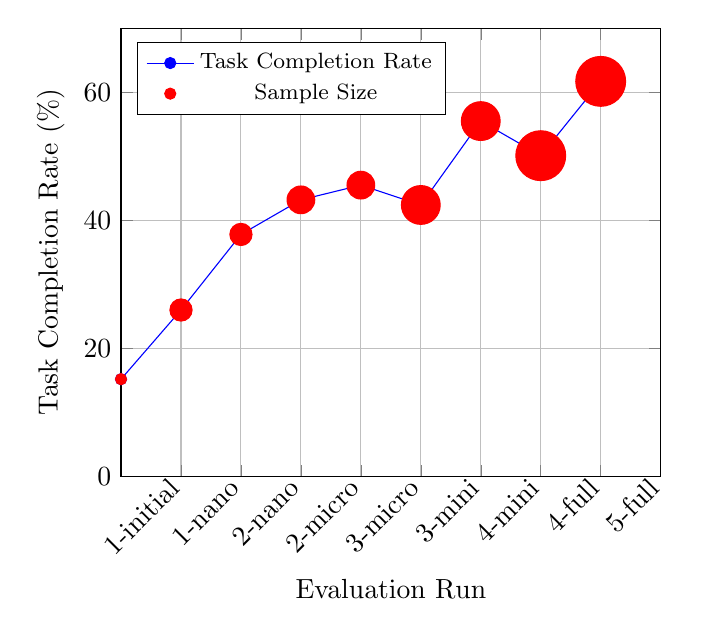
\begin{tikzpicture}
        \begin{axis}[
            xlabel=Evaluation Run,
            ylabel=Task Completion Rate (\%),
            xmin=0, xmax=9,
            ymin=0, ymax=70,
            xtick={1,2,3,4,5,6,7,8,9},
            xticklabels={1-initial, 1-nano, 2-nano, 2-micro, 3-micro, 3-mini, 4-mini, 4-full, 5-full},
            xticklabel style={rotate=45,anchor=east},
            grid=major,
            legend pos=north west,
            legend style={font=\footnotesize},
        ]
        % Line plot for task completion rate
        \addplot[color=blue, mark=*] table [x index=0, y index=1] {
            0 15.2
            1 26.0
            2 37.8
            3 43.2
            4 45.5
            5 42.4
            6 55.5
            7 50.1
            8 61.7
            
        };
        \addlegendentry{Task Completion Rate}

        % Scatter plot for sample size (with varying marker size)
        \addplot[only marks, mark=*, color=red, scatter,
            scatter src=explicit symbolic,
            scatter/classes={
                22={mark size=2pt},
                44={mark size=4pt},
                90={mark size=5pt},
                190={mark size=7pt},
                812={mark size=9pt}
            }] table [x index=0, y index=1, meta index=2] {
            0 15.2 22
            1 26.0 44
            2 37.8 44
            3 43.2 90
            4 45.5 90
            5 42.4 190
            6 55.5 190
            7 50.1 812
            8 61.7 812
        };
        \addlegendentry{Sample Size}
        \end{axis}
    \end{tikzpicture}
    \caption{Evolution of CUGA Architecture Performance. The graph illustrates the task completion rate (\%) across different evaluation runs.  Each run is denoted by the iteration and the dataset sample name.  The size of the markers corresponds to the sample size where in each iteration we validate performance gains on the previous sample, as well as enlarge the sample to learn about new failures.  Note that in some instances, increasing the sample size led to a minor reduction in performance, reflecting the approximation inherent in our sampling strategy. Overall, the graph demonstrates a clear trend of improvement in task completion rate over time, showcasing the effectiveness of our iterative refinement process.}
    \label{fig:cuga_evolution}
\end{figure}


\section{Lessons Learned, Challenges, and Roadmap}

\paragraph{Methodology and Tools:} Our iterative development methodology, coupled with smart evaluation and analytics tools, has been crucial for rapid progress and achieving state-of-the-art results cost-effectively.  These tools have enabled us to effectively assess failures and identify areas for improvement. However, the process of finding, classifying, and aggregating root causes of failures within agentic trajectories remains labor-intensive, even with current tooling. Automating some of this manual effort, perhaps by leveraging AI agents, could significantly accelerate the development of agentic systems and potentially pave the way for fully autonomous evolution.  Another interesting research opportunity lies in the area of smart regressions and how to evaluate individual agents within a full agentic system.  Currently, best practices and lessons learned in this area are not widely shared. We hope this paper contributes to the community by sharing our experiences.  Within IBM, we are leveraging insights, methodologies, and tools from initiatives like IBM CUGA and others, integrating and hardening them into the observability and analytics layers of the IBM Agentic Middleware platform. This will allow clients to benefit from these capabilities at a product-grade level.

\paragraph{Evaluating Generalist Agents on Realistic Benchmarks:} Creating and maintaining effective benchmarks is a significant challenge.  Many existing benchmarks are developed within academic settings, reflecting the tasks and tools readily available to researchers.  While valuable, these benchmarks often lack the complexity and nuances of real-world scenarios.  A promising recent effort, TheAgentCompany \cite{xu2024theagentcompanybenchmarkingllmagents}, aims to address this by simulating more realistic tasks and incorporating human-agent communication.  However, current benchmarks often focus on "happy path" scenarios and neglect critical aspects like safety, especially for agents interacting with enterprise systems, applications, and APIs.  They typically do not evaluate agent behavior in exceptional circumstances or when human-in-the-loop interaction is required.  A notable effort in this direction is STWebAgentBench \cite{levy2024st}, which extends WebArena by incorporating safety and policy adherence measurements alongside task completion.  Ultimately, realistic benchmarks should mirror the specific environments, policies, and enterprise use cases of individual organizations.  At IBM Research, we plan to further evolve CUGA to be a safe and policy-compliant, and to be a collaborative and trustworthy AI agent with human-in-the-loop support.  Furthermore, we plan to evaluate CUGA on several leading benchmarks. These benchmarks combine multiple tools, desktop applications, coding, and APIs. We will also contribute to the community's efforts in developing more comprehensive evaluation frameworks.

\paragraph{Learning, Customization, and Adaptation:}  Traditional system development relies on programming languages and low-code/no-code tools to build and test systems according to specifications defined in requirements documents.  Agentic systems offer a radically different paradigm.  Agents can potentially learn to perform tasks much like humans: by studying documentation and policies, receiving instructions, observing expert behavior, analyzing videos, and through interactive discovery and safe exploration.  Emerging research suggests this vision is within reach.  At IBM Research, we have begun experimenting with methods to enable CUGA to learn from unstructured documents and empower non-technical users to configure and customize its behavior to meet their specific needs.


\paragraph{Smaller and Open Models:} While our current state-of-the-art results are based on a frontier model, this choice was primarily driven by time efficiency, allowing us to rapidly iterate on our agentic architecture for the WebArena benchmark.  We recognize the significant advantages of smaller and open models, particularly in terms of accessibility, affordability, privacy, efficiency, and cost.  We have initiated experiments evaluating our architecture with these models and plan to publish a comprehensive evaluation of our findings upon completion.

\section{Conclusion}

In this paper, we have presented the current status of our work on developing IBM CUGA.  We detailed the iterative evolution of our agentic architecture, the methodology and tools that facilitated rapid learning and cost-effective improvements, and key lessons learned and challenges ahead. Our results demonstrate the effectiveness of our approach, achieving state-of-the-art performance on the WebArena benchmark. We believe that our contributions provide valuable insights and practical guidance for the community, paving the way for future advancements in the field of enterprise-ready agentic AI systems.

% \printbibliography

% References (if you are using BibTeX)
\bibliographystyle{plain}
% \bibliographystyle{plainnat}
\bibliography{references} % Ensure that you upload your .bib file

\end{document}
